%% This is an example first chapter. You should put chapter/appendix that you
%% write into a separate file, and add a line \include{yourfilename} to
%% main.tex, where `yourfilename.tex' is the name of the chapter/appendix file.
%% You can process specific files by typing their names in at the 
%% \files=
%% prompt when you run the file main.tex through LaTeX.
\chapter{Background and Motivation}

\begin{flushright}
\textit{``The mathematician's patterns, like the painter's or the poet's 
must be beautiful; the ideas like the colours or the words, must fit 
together in a harmonious way. Beauty is the first test: there is no 
permanent place in the world for ugly mathematics."
}
G. H. Hardy \cite{hardy}
\end{flushright}


In order to illustrate the creative potential of algorithmic craft, it is useful to examine its contents: computational design, digital fabrication and craft. Each of these disciplines have distinct strengths and limitations. Through their convergence, new, compelling forms of creation become possible. In computational design, the abstract qualities of computation provide a powerful way of thinking about design. With appropriate programming, a computer can embody any conceivable process \cite{mateas}. Similarly, computational design can be applied to any design domain, be it physical, visual, sonic, or interactive. Although individual applications of computational design often consider material properties that are relevant to a specific domain, computational design does posses an inherent connection to the material world. Craft on the other hand is closely linked to materiality. Craftspeople work in close contact with the physical world and craft artifacts and processes are directly informed by material properties. Digital fabrication provides a connection between the abstraction of computational design and the material domain of craft, by converting digital concepts to physical forms. In the following section I discuss the properties of computational design, digital fabrication and craft in greater detail and describe connection points between each discipline.

 \begin{center}
\begin{figure}[h!]
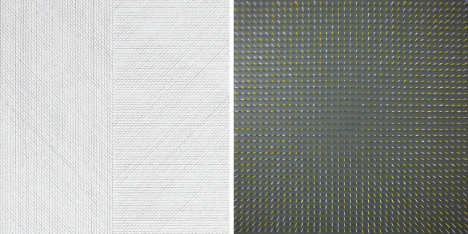
\includegraphics[width=\columnwidth]{images/wall_drawings.jpg}
\caption{Wall drawings by Sol Lewitt. From left to right: Wall Drawing 19: A wall divided vertically into six equal parts, with two of the four kinds of line directions superimposed in each part (1969), Wall Drawing 38 (Detail): Tissue paper cut into 1.5-inch (4 cm) squares and inserted into holes in the gray pegboard walls. All holes in the walls are filled randomly (1970).}
\label{fig:wall_drawings}
\end{figure}
\end{center}

\section{Computational Design}\label{sec:computational_design}
As previously mentioned, computational design can refer to a range of design practices that incorporate computational processes. Computational processes are explicit patterns of rules that can manipulate data \cite{abelson}. Computer programs are description of computational processes in a format that is readable by a computer. My focus in computational design is the process of using computation processes to create visual forms and patterns. Because computational design usually requires the designer to write programs, it is possible to mistake the practice of computational design as a technical skill rather than a way of thinking \cite{reas}. It is true that computational design does require a degree of technical expertise; practitioners must be able to write and read code. Despite this requirement, computational design is better represented as a way of applying procedural thinking to a design task. Rather than producing specific design representations, the designer authors a set of rules that define a system capable of producing many outcomes. Designs are presented in abstract terms, resulting in the potential to create multiple variations that share a set of constraints. One of the challenges of computational design is in authoring guidelines that effectively produce solutions within the desired design space. Presented as an ordered set of instructions, these guidelines constitute an algorithm. Arguably, it is possible to engage in computational design without using a computer. The artist Sol Lewitt created a number of artworks consisting of a set of instructions that dictated the constraints of an artwork:

\begin{quotation}
WORK FROM INSTRUCTIONS (1971):
\\USING A BLACK, HARD CRAYON DRAW A TWENTY INCH SQUARE.
\\DIVIDE THIS SQUARE INTO ONE INCH SQUARES.
 \\WITHIN EACH ONE INCH SQUARE, DRAW NOTHING, OR DRAW A DIAGONAL STRAIGHT LINE FROM CORNER TO CORNER OR TWO CROSSING STRAIGHT LINES DIAGONALLY FROM CORNER TO CORNER.
\end{quotation}

 The resulting piece would vary depending on how the instructions were interpreted by the people executing them. Many of his other artworks contained the instructions for producing them in the title of the piece (figure:\ref{fig:wall_drawings}.) Using a computer to execute computational design algorithms as opposed to human beings greatly accelerates the process of execution, and supports a non-linear design process. The specific affordances of computational design are as follows:
 
\begin{itemize}
\item \textbf{Precision:} Computation supports high levels of numerical precision with relatively little effort on the part of the designer.

\begin{center}
\begin{figure}[h!]
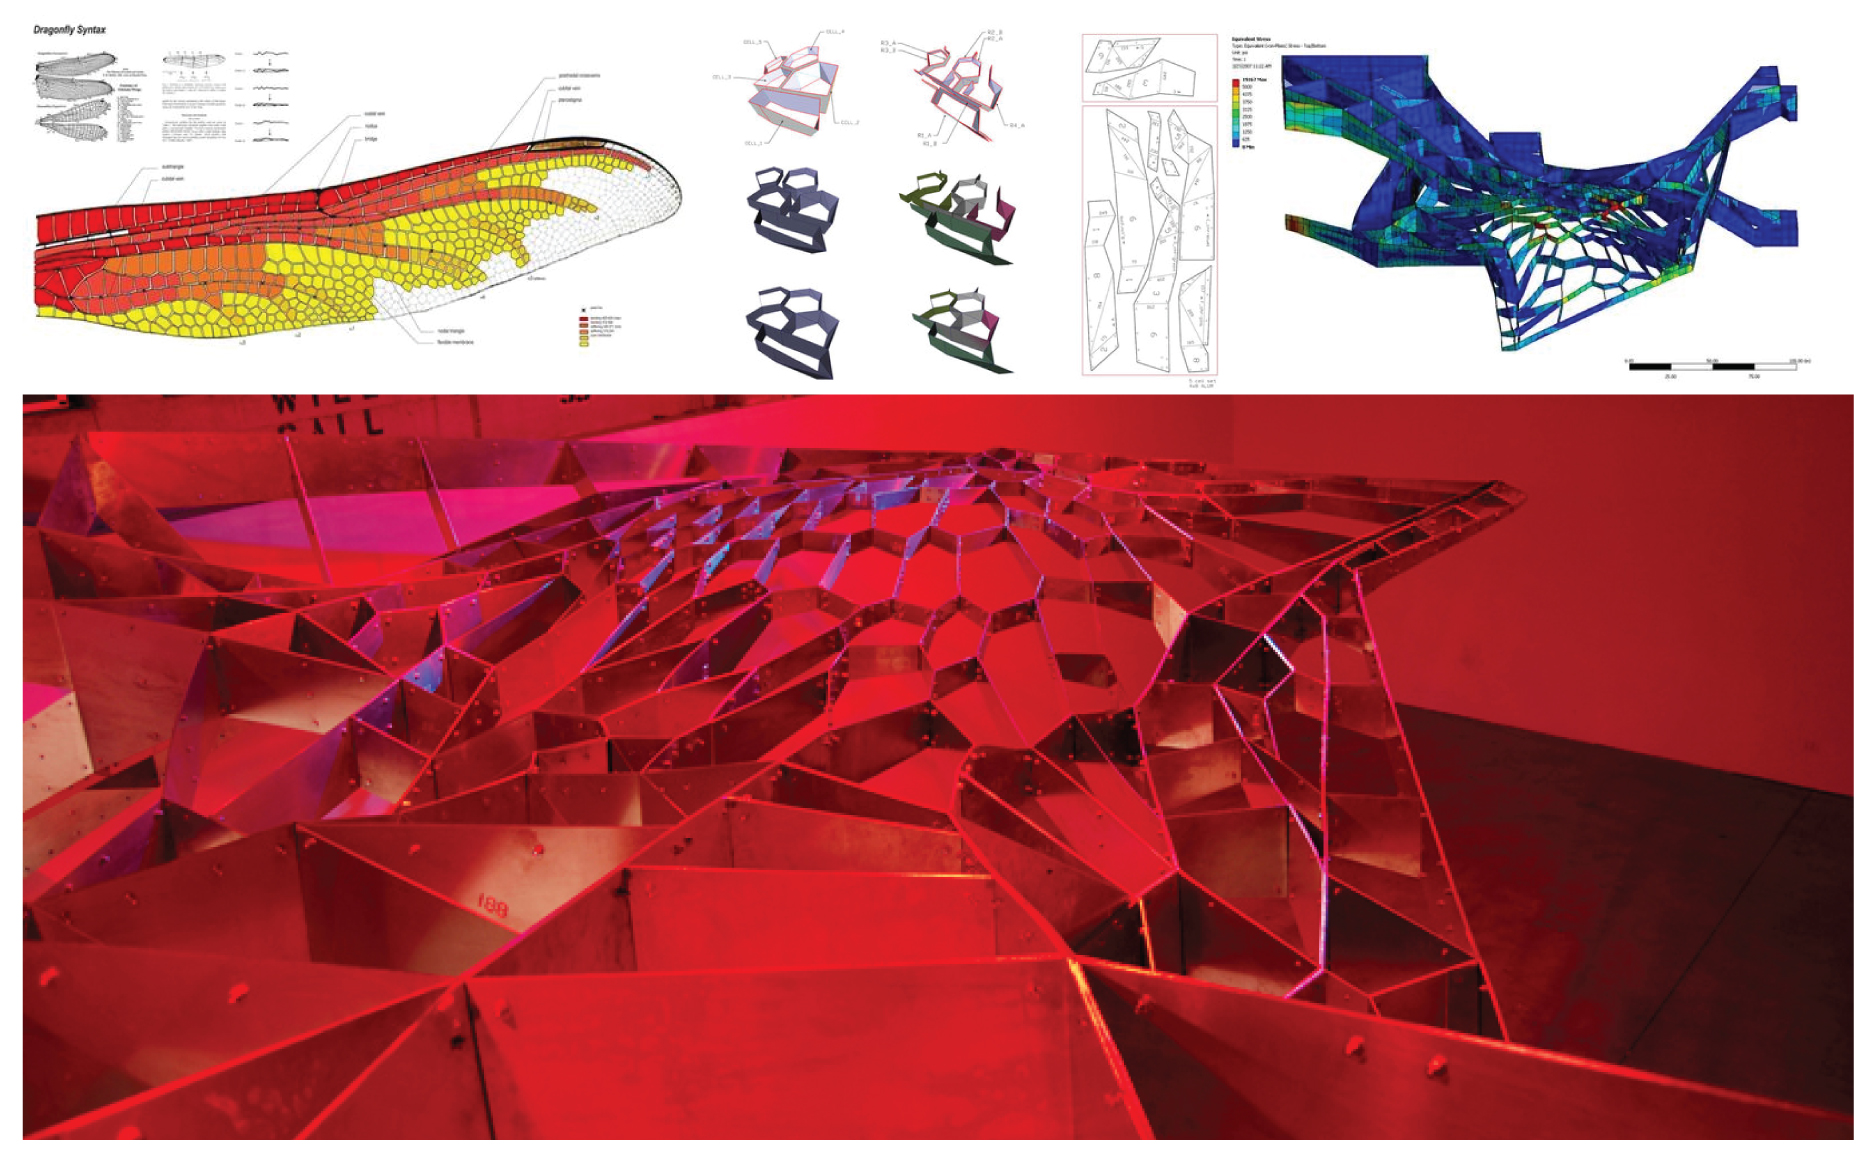
\includegraphics[width=\columnwidth]{images/dragonfly.jpg}
\caption{Dragonfly by EMERGENT/ Tom Wiscombe (2007). Installation. Inspired by the structure of a dragonfly wing, this installation was shaped in by a set of parameters including gravity, specific support points and flat material properties. The structure was generated based on support and loading data, which was run through a feedback loop, producing a design which supported both the performance criteria and a novel variation of form \cite{dunn}. }
\label{fig:dragonfly}
\end{figure}
\end{center}

\item \textbf{Visual Complexity:} Computational design supports the creation and transformation of complex patterns and structures through rapid automation and iteration which allows for the combination and manipulation of large numbers of simple elements in a structured manner. 

\begin{center}
\begin{figure}[h!]
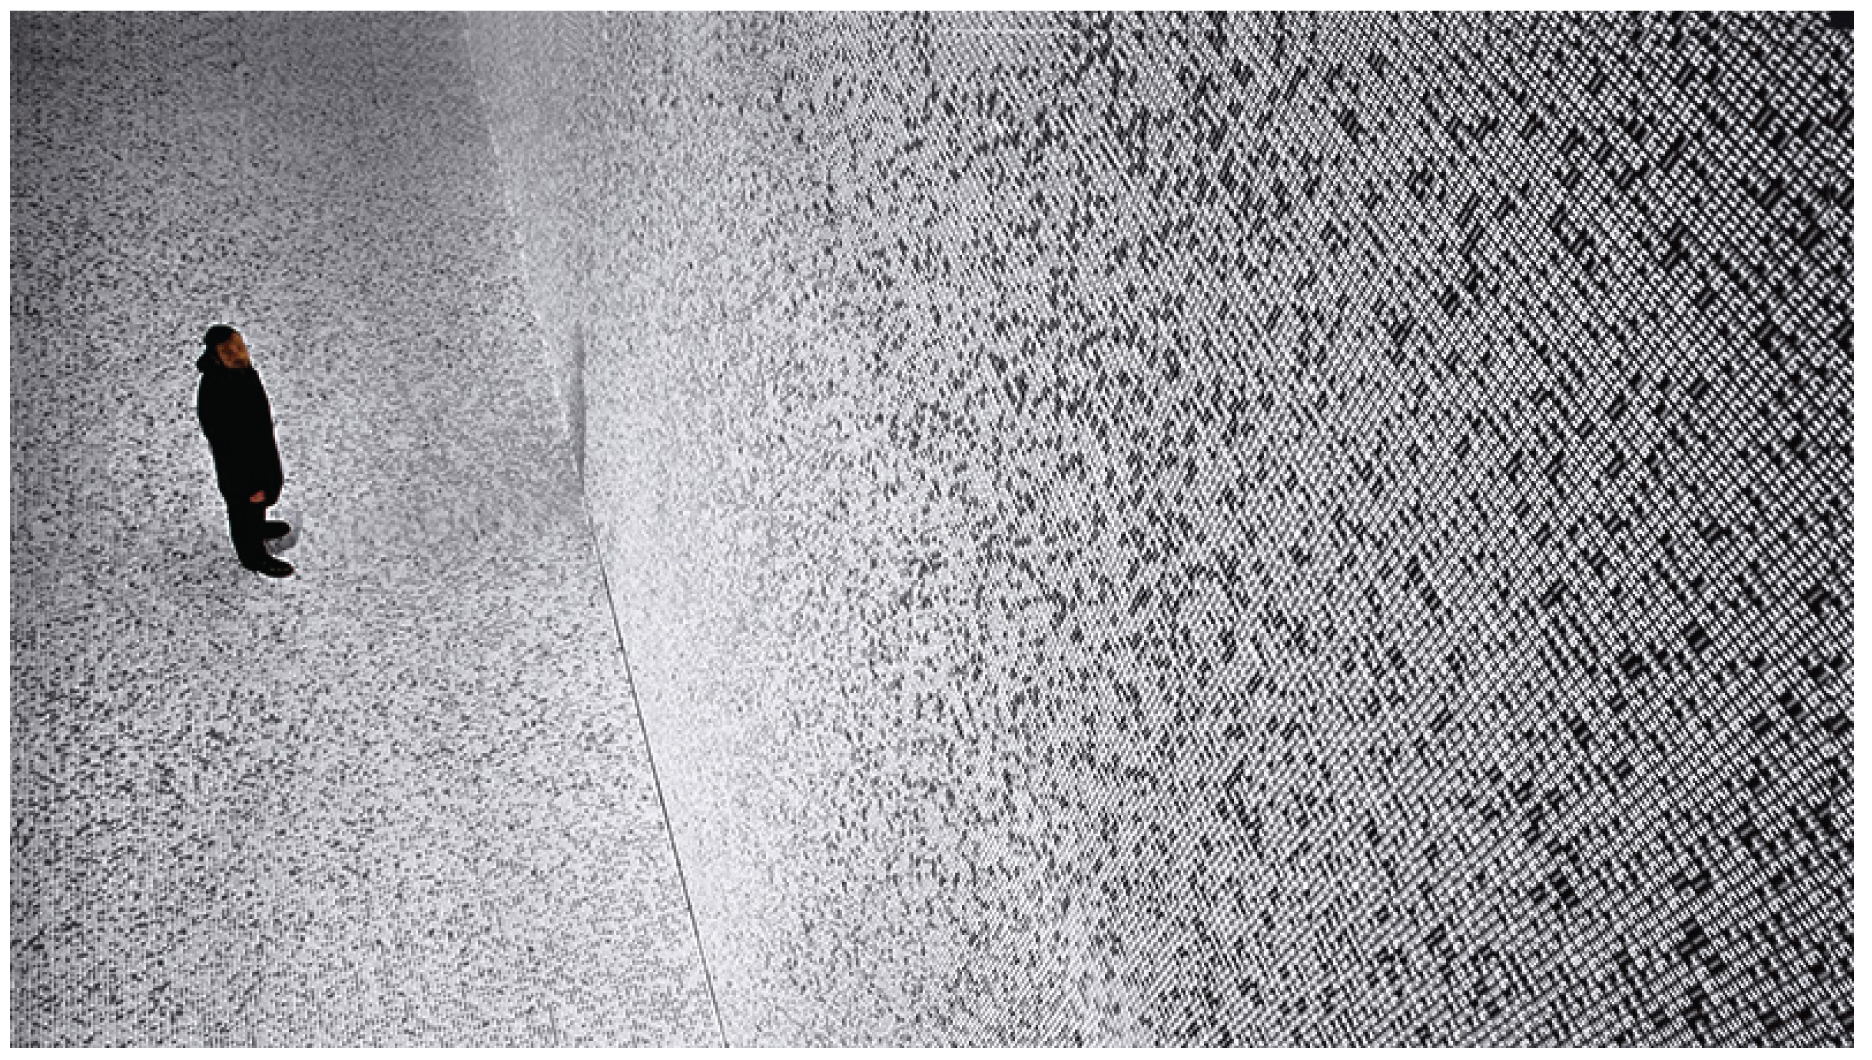
\includegraphics[width=\columnwidth]{images/ikeda.jpg}
\caption{data.tron by Ryoji Ikeda (2008). Dynamic computer visual and sound installation. Each pixel of the visual image is dynamically calculated as a visualization of data from hard drive errors and software code. \cite{ikeda_website}. }
\label{fig:ikeda}
\end{figure}
\end{center}

\item \textbf{Generativity and randomness:} Computation allows for the programmer to create algorithms which when run, allow for the computer to autonomously produce unique and often unexpected designs.

 \begin{center}
\begin{figure}[h!]
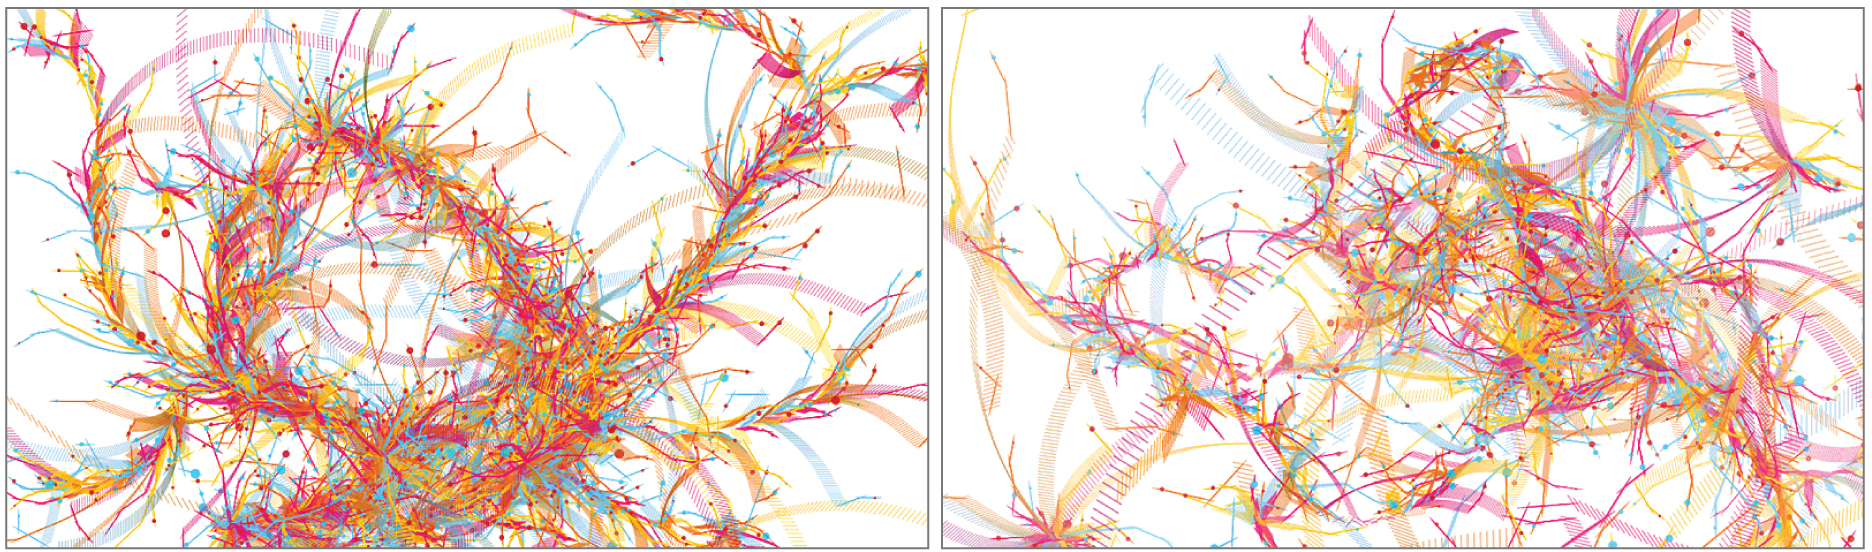
\includegraphics[width=\columnwidth]{images/marius_watz.jpg}
\caption{Abstract01.js by Marius Watz (2010). Interactive. The piece is comprised of a java script program that autonomously creates unique abstract compositions based on a set of visual guidelines specified by the artist \cite{watz_website}.}
\label{fig:marius_watz}
\end{figure}
\end{center}

\item \textbf{Parameterization:} Computation allows users to specify a set of degrees of freedom and constraints of a model and then adjust the values of the degrees of freedom while maintaining the constraints of the original model.

\begin{center}
\begin{figure}[h!]
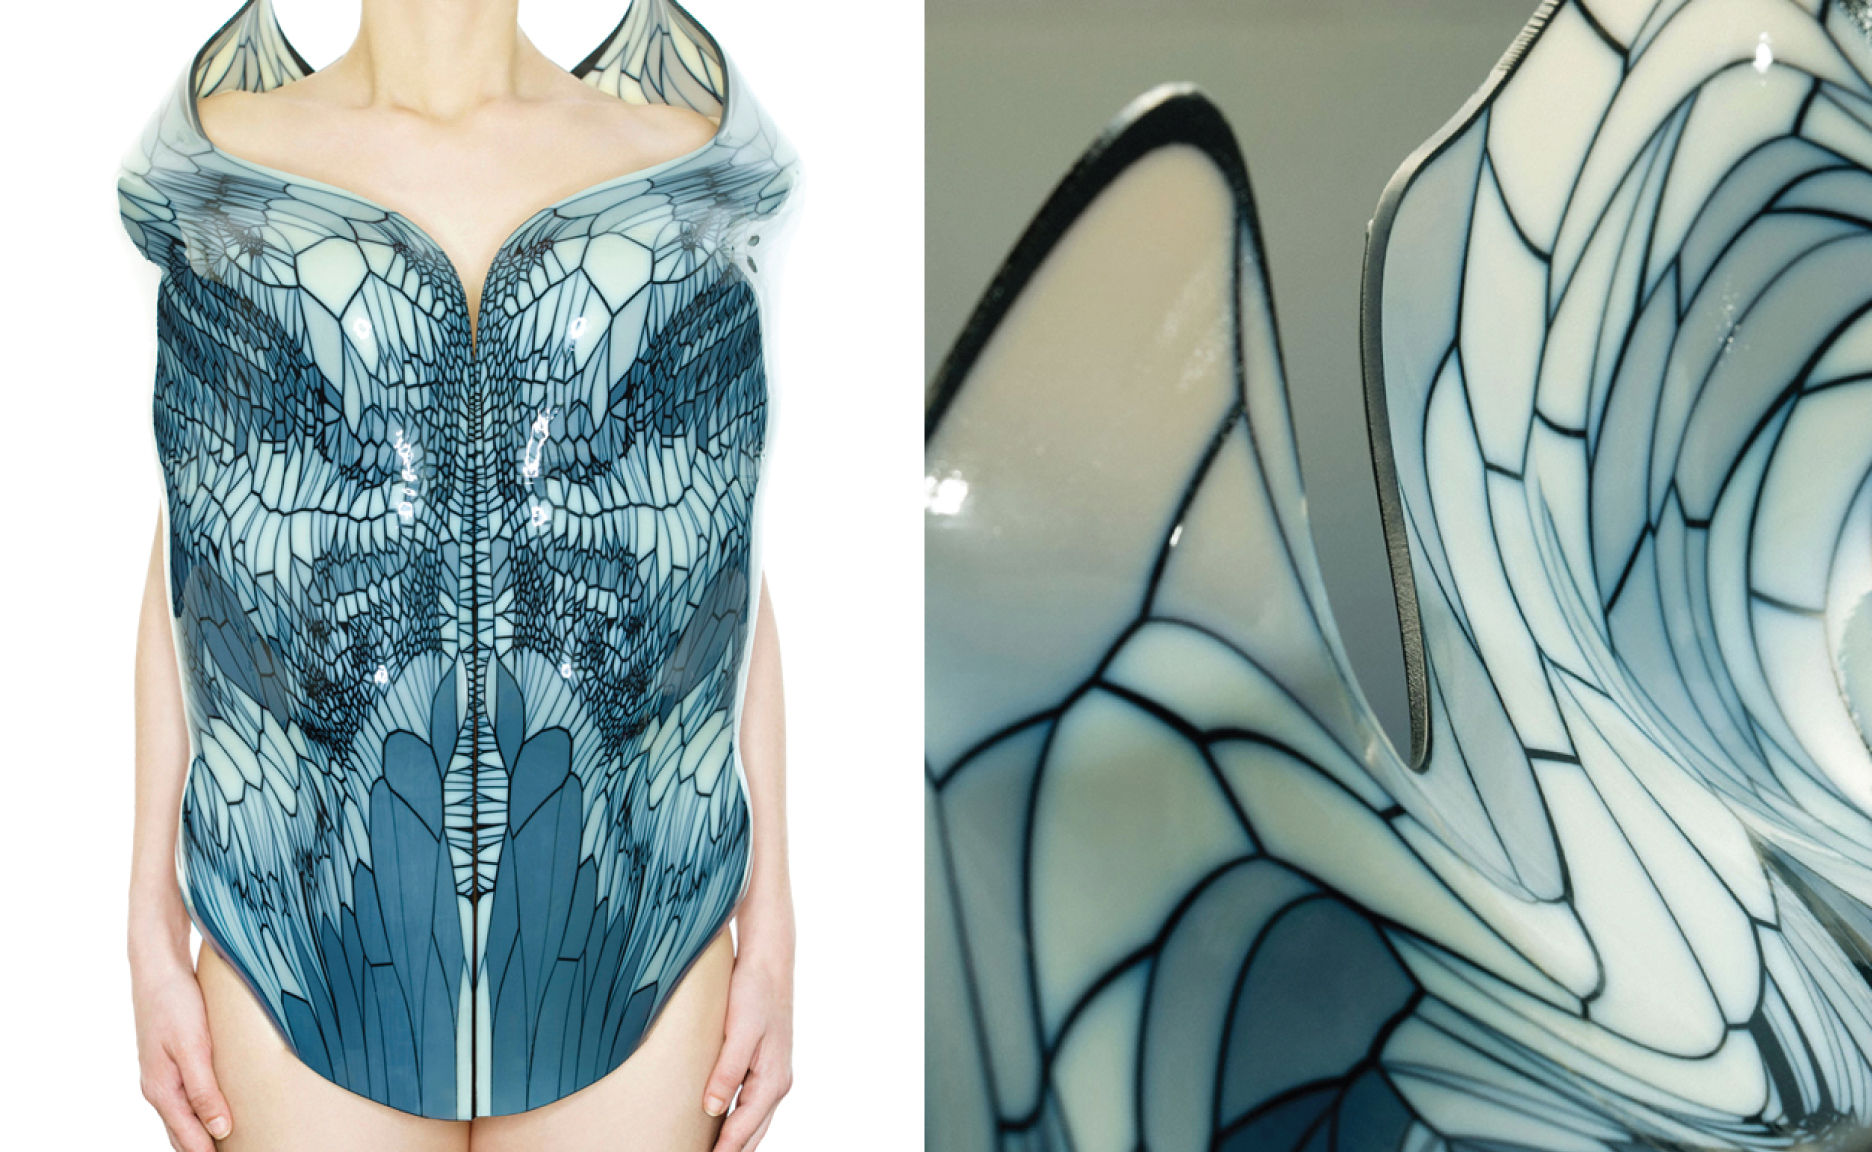
\includegraphics[width=\columnwidth]{images/arachne.jpg}
\caption{Arachn\`{E}Armor / Corset by Neri Oxman (2012), Digital Materials Centre Pompidou, Paris, France. The form of the web on the piece is determined by the anatomical location of a person's rib cage \cite{oxman_arachne}. }
\label{fig:arachne}
\end{figure}
\end{center}

\item \textbf{Documentation and remixing:} Computationally generated designs are generated by a program, a document which can be shared with and modified by other designers. These programs also serve as a form of documentation of the design process itself. 

\begin{center}
\begin{figure}[h!]
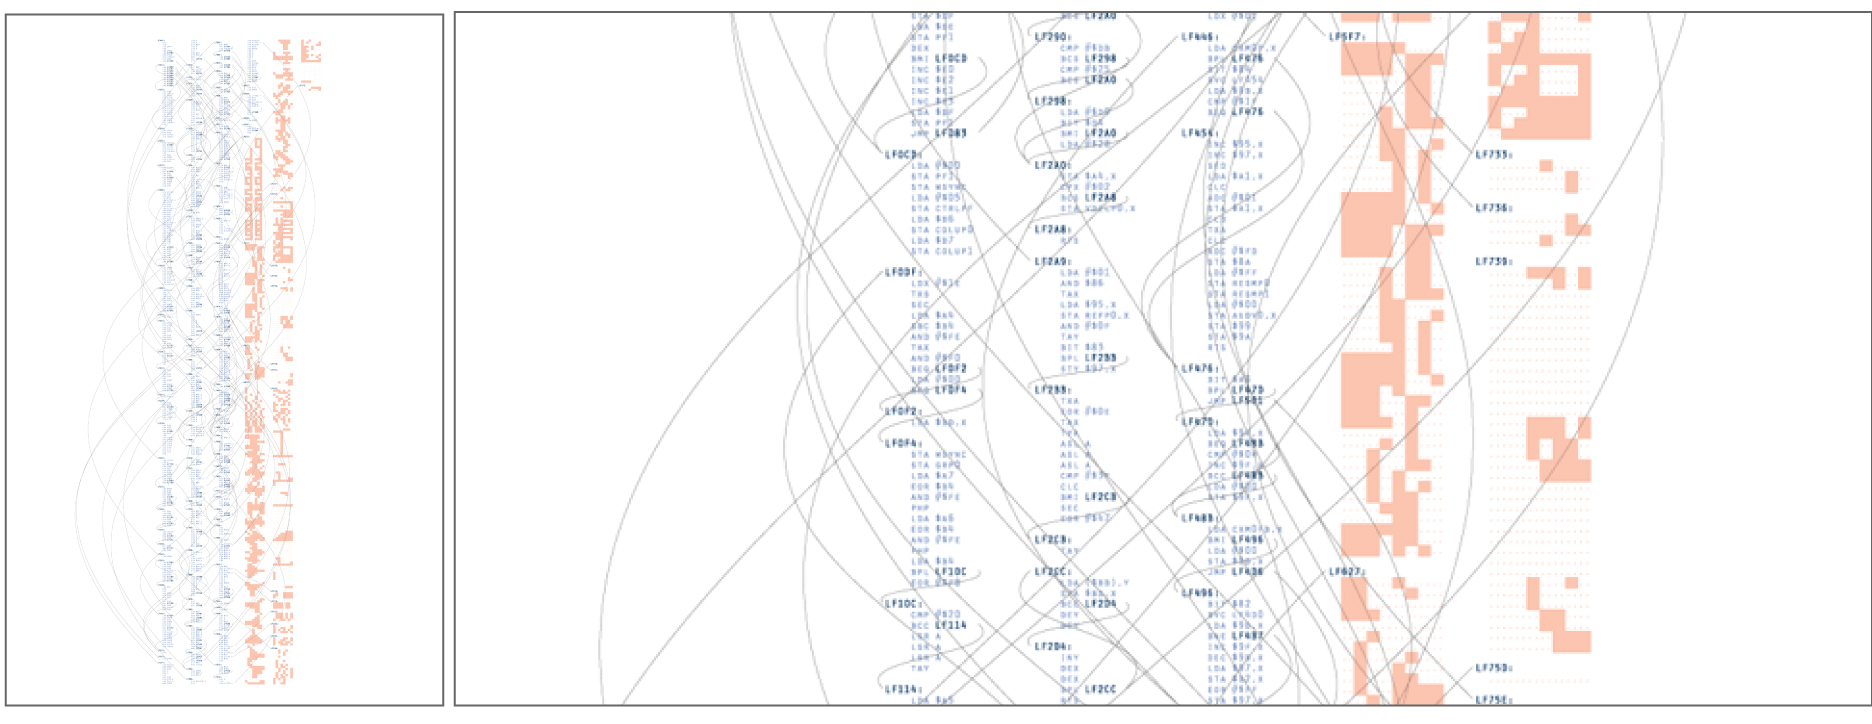
\includegraphics[width=\columnwidth]{images/distillamap.jpg}
\caption{Contra from Distellamap Series by Ben Fry (2005) Digital Print. The Distellamap series translates the code from a number of Atari2600 video games into a series of visualizations. Assembly code from each cartridge is shown in blue, with connection lines denoting ``go to" statements. Data is shown in orange \cite{fry_website}. }
\label{fig:arachne}
\end{figure}
\end{center}

\end{itemize}	

In combination with these affordances however, computational design also contains a number of unique challenges:
\begin{itemize}
\item \textbf{Formalizing complex problems} As design problems grow in complexity, formalizing the problem in a manner that can be expressed programmatically becomes challenging. Writing an algorithm to generate a single visual pattern is simple, however writing a program to incorporate that pattern into the design of a complex assembly is difficult. 
\item \textbf{Creating singularities:} A designer will often choose to deviate from a set pattern or structure at specific points in order to create a special emphasis in that area. Because computational design is governed by a systematized ruleset, the methods of breaking these rules at arbitrary points is are often unclear and tedious to implement. 
\item \textbf{Selecting a final design:} The systematic approach to computational design gives the designer the ability to produce extremely large numbers of solutions to a single design problem. While this is useful in situations where multiple solutions are required, when a single design must be chosen, the process of deciding on a solution is often difficult and sometimes arbitrary, especially if the decision is based on aesthetic criteria.
\end{itemize}

\section{Digital Fabrication} Although computational design is performed on a computer, the artifacts generated by computational design are not restricted to the screen. Digital fabrication technology provides the opportunity to translate digital files to physical form.  Digital Fabrication is supported through computer aided design (CAD) technology. CAD involves the use of a software tool to design an object. Some form of CAD file is generally required to control a digital-fabrication machine \cite{dunn}. Digital Fabrication is the process of using computer-controlled machines to fabricate objects specified by a digital tool path. Digital fabrication shares many of the affordances of computational design. In particular, it allows for the creation of physical objects with a high degree of complexity, without skill in craft or extensive manual labor. Digital fabrication also allows for the rapid production of small volumes of similar or identical objects. Also, because the artifacts produced through digital fabrication are derived from digital files, anyone with access to the file, and a similar fabrication machine can potentially create a copy of the object, or remix that object with others. 

There are two primary forms of digital-fabrication manufacturing, additive and subtractive. Subtractive processes machine a part by removing pieces from the original material and include tools like laser cutters, computer numerically controlled (CNC) milling machines and vinyl cutters. Additive processes create a part by incrementally adding successive layers of material. 3D printers are most commonly associated with additive manufacturing, however ink jet printers and CNC embroidery machines also fit this definition. Although advances in additive technology are occurring at a rapid pace, at this point the material options for 3D printing are limited. Most 3D printers can output objects in plastics, ceramic and metal composites \cite{dunn}. Low-end 3D printers are even more constrained, and can only print in ABS plastic. Additive manufacturing is also extremely expensive and often constrained to small build volumes.\todo{reference wood printing 3D printers, other novel 3D printing techniques} 

\todo{insert picture of 3d printed and subtractive pieces}

Unlike most 3D printing technology, subtractive processes can work with a wide range of materials \cite{dunn}. Laser cutters work well with materials such as wood, leather, paper and cloth. Vinyl cutters can also be used on cloth, paper, in addition to adhesive vinyl. Milling machines can cut parts from plastic, foam, metal and wood. In specialized cases these machines can also be modified to function in an additive manner with custom attachments. An example is the adaptation of a 3-Axis ShopBot to function as a threading device to facilitate part of the construction of a Silk Pavilion, created by the Mediated Matter Group at MIT (figure \ref{fig:pavilion} \cite{pavilion}.) Large-scale subtractive fabrication machines also make it possible to work at a larger scale than additive processes \cite{dunn}.

\begin{center}
\begin{figure}[h!]
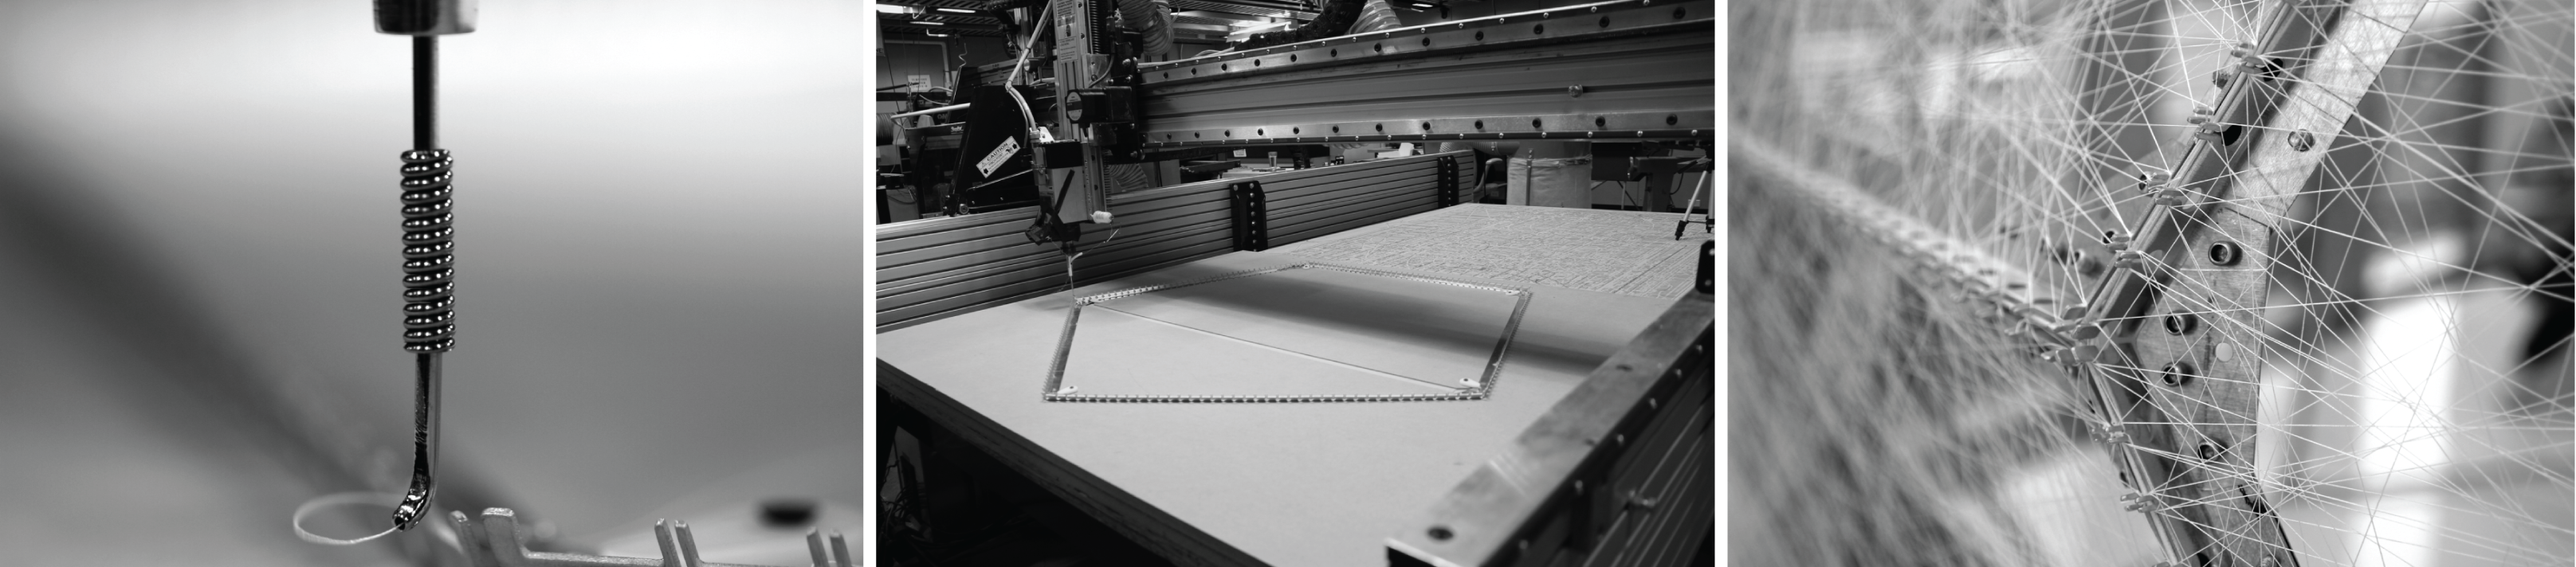
\includegraphics[width=\columnwidth]{images/pavillion_shopbot.png}
\caption{3-axis CNC milling machine adapted as CNC deposition tool using a custom threading tool. (Part of the Silk Pavilion Fabrication process)}
\label{fig:pavilion}
\end{figure}
\end{center}

Widespread access to digital fabrication is growing. Digital fabrication machines are rapidly decreasing in price and increasing in availability \cite{gershenfeld}. This trend has allowed an increasing number of individuals and small groups to gain access to sophisticated manufacturing technologies, and signaled the growth of personal fabrication \cite{lipson}. Consumer 3D printers can now be purchased at prices ranging from \$1,000-\$3,500 dollars. Small scale laser cutters and milling machines are available at prices ranging from \$3,000 to \$5,000. \todo{add in citations for prices} In addition, other groups are producing open-source versions of commercial fabrication equipment, like the MTM Snap CNC-milling machine, the LaserSaur laser cutter and the RepRap 3D printer. Though these devices require additional levels of expertise to assemble, they point to to exciting future developments in affordable and open forms of digital fabrication. Machines like inkjet printers and craft CNC-vinyl cutters also function as personal fabrication devices and are extremely accessible and affordable. 

There are also options for individuals without direct ownership of a fabrication machine. Community hacker spaces like Artisans' Asylum in Cambridge, NYC resistor in New York and Noisebridge in San Francisco, and organizations like the FabLab network provide access to shared digital fabrication facilities. Online services like Shapeways, Ponoko and SpoonFlower offer on-demand fabrication services to individual consumers for a variety of materials and machining processes. 

The rise of personal fabrication is often viewed as a component of the maker movement \cite{anderson}. The maker subculture is a technology-literate community that is engaged in the production of devices and artifacts in line with the do-it-yourself (DIY) philosophy. While maker culture has a strong technological focus, it also encompasses hobbyist craft techniques and materials. MakerFaire, one of the predominate maker culture events, showcases a range of DIY practice across science, engineering, art, and craft \cite{maker_faire}. Some of the primary tenants of the maker movement correspond to values frequently expressed in craft.

\section{Craft}
The cultural connotations of craft have varied throughout history. Once the primary means of producing functional objects, the role of craft changed following the industrial revolution. In the face of mechanized production, hand skills became less central to production, and design, traditionally unified with the role of the artisan emerged as a separate discipline \cite{abstracting_craft}. Despite the emergence of mass production, craft has endured, both as a recreational pursuit, and as set of valued artisanal practices. My personal interest in craft focuses on three specific qualities: materiality, pleasure and craftsmanship.
\begin{itemize}
\item \textbf{Materiality:} One primary aspect of craft involves the manipulation of physical materials \cite{on_craft}. Working with physical materials requires the use of one's hands, and is often an intuitive process. When we craft, we experience the feel of the paint brush moving across the canvas, the carving knife through a piece of wood, a needle through cloth, or our fingertips pressing into clay. The decisions we make in the craft process are altered by the feel of working with the material. 

\todo{insert picture of material evidence of craft (clay?)}

\item \textbf{Pleasure:} One of the responses to industrialism was the Arts and Crafts movement, initiated primarily by William Morris, and inspired by the writings of John Ruskin. 
The arts and crafts movement sought to restore the aesthetics and practices of traditional craftsmanship, in response to the negative aesthetic effects and working conditions of industrialism. Fundamental to the arts and crafts movement was the notion that the act of creating beautiful artifacts with one's hands was a pleasurable, and essential human experience \cite{abstracting_craft}. This emphasis on pleasure is retained in conceptions of craft today.

\item \textbf{Craftsmanship:} Although not all craft is functional, many forms of traditional craft, including sewing, pottery, and carpentry can be applied the creation of useful objects. In addition to this functionality, craft often emphasizes the importance of beauty in the form and ornamentation of objects. I use the term craftsmanship to describe the successful unification of aesthetics and utility in a single artifact. 
\end{itemize}

\todo{insert picture of decorative object from arts and craft movement}

\section{Algorithmic Craft}
Algorithmic craft is the combined use of computational design, digital fabrication and hand craft. The merging of the properties of craft with computational design and digital fabrication allows for a creative practice that exhibits the variability and complexity of computation, the precision and repeatability of fabrication and the material, functional and aesthetic concerns of craft. Algorithmic crafting allows individuals use programing and digital fabrication as a means of pleasurable and useful creative expression. In addition, algorithmic craft encourages the incorporation of the values of artisans and craftspeople in development of new methods of digital fabrication and computational design tools, paving the way for new forms of innovation in these fields. Below I describe several examples of combing digital fabrication and craft, and computational design and craft respectively.

\subsection{Digital Fabrication and Craft}
Objects that emerge from a combined practice of digital fabrication and craft are often characterized by their physical craftsmanship, technical mastery and exceptional aesthetic. Practitioners in this space blur the boundaries between engineer, designer and artisan. One of the advantages of merging craft and digital fabrication is that it ensures that machine-produced artifacts retain their personal history. For his Hybrid Reassemblage pieces, Amit Zoran blended handcraft techniques like basket weaving and slip casting with 3D-printed forms. The process resulted in artifacts that retained the evidence of hand production in conjunction forms made possible through computational design and digital fabrication (figure: \ref{fig:hybrid})\cite{zoran}.

\begin{center}
\begin{figure}[h!]
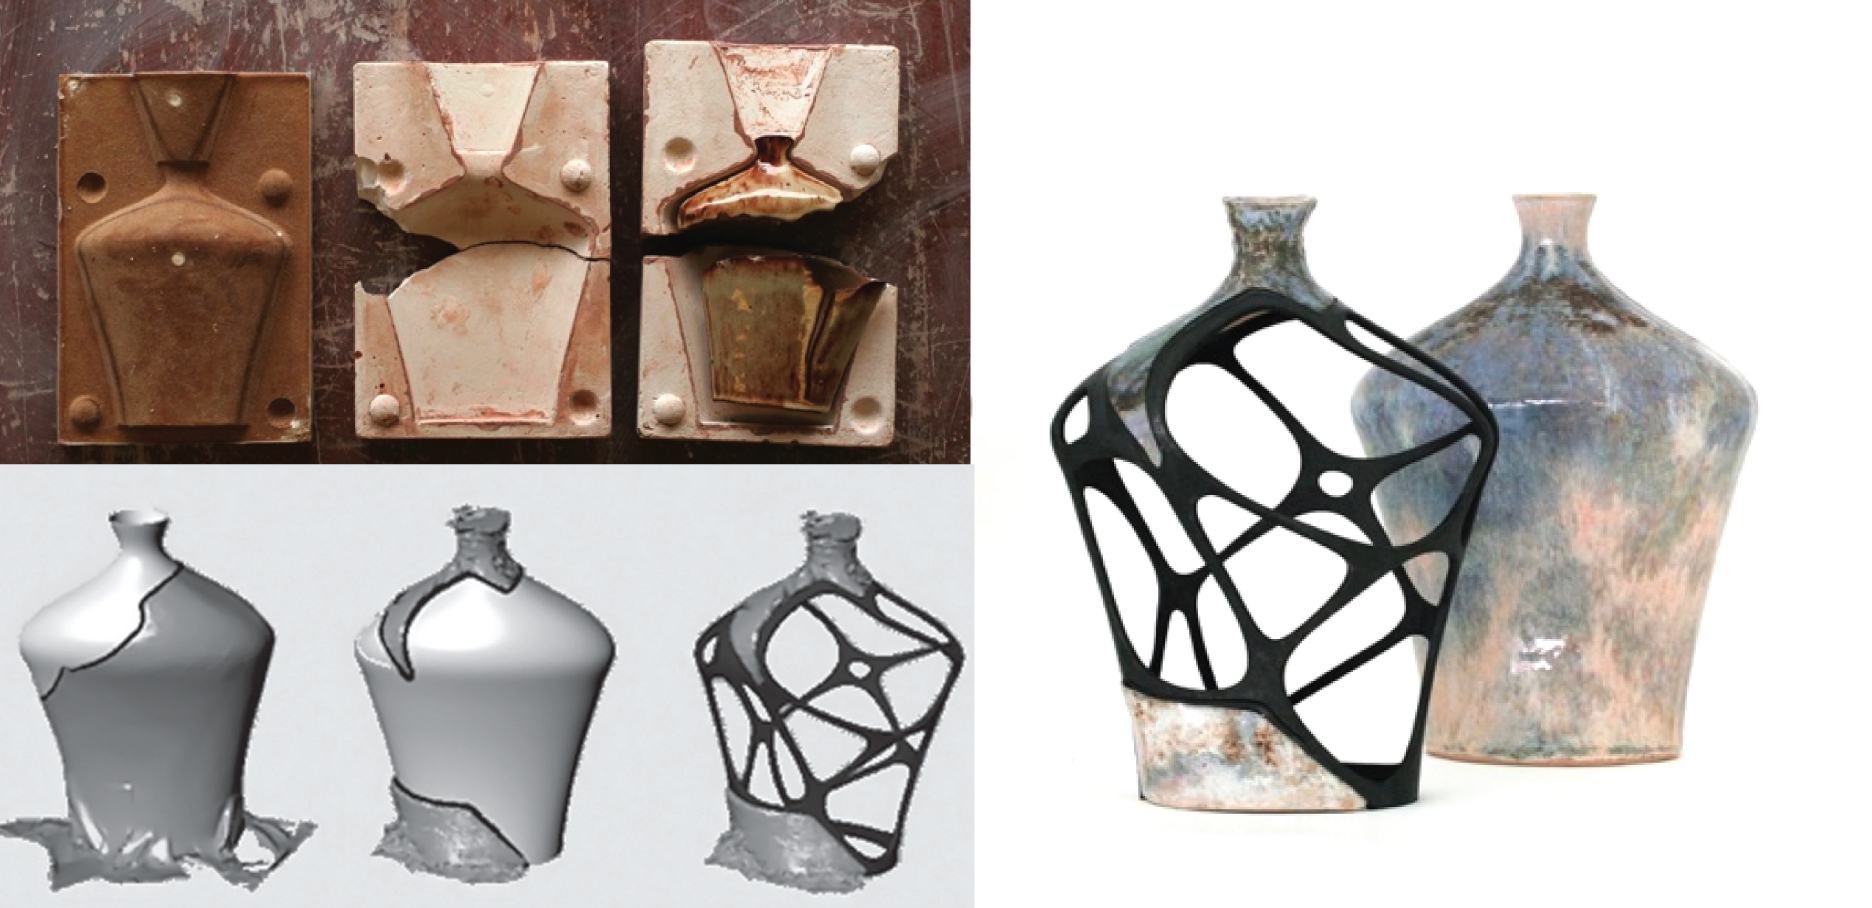
\includegraphics[width=\columnwidth]{images/amit.jpg}
\caption{A selection of vases from the Hybrid Reassemblage series by Amit Zoran (2010). Glazed
ceramic, SLS nylon element, epoxy glue and black spray paint.}
\label{fig:hybrid}
\end{figure}
\end{center}

Another advantage of combining digital fabrication and craft is that it affords openness and flexibility in the design of functional components. Peter Schmitt's plywood servo is a re-designed RC servo in laser-cut plywood. Although the parts of the servo are digitally designed,  after fabrication the completed piece is constructed by hand. This process of hand construction gives the designer greater control in the form-factor and aesthetic of the servo, while maintaining its functional qualities \cite{plywood_punk}. As one sample application, the plywood servo was incorporated into a custom drawing machine called the Audiograph, producing a surprising and novel object with no precedent. The objective of the audio graph was to create a device with an appearance that was drastically different to customary home electronics and explore people's reaction to it in a home setting (figure: \ref{fig:plywood_servo})\cite{schmitt_thesis}. 

\begin{center}
\begin{figure}[h!]
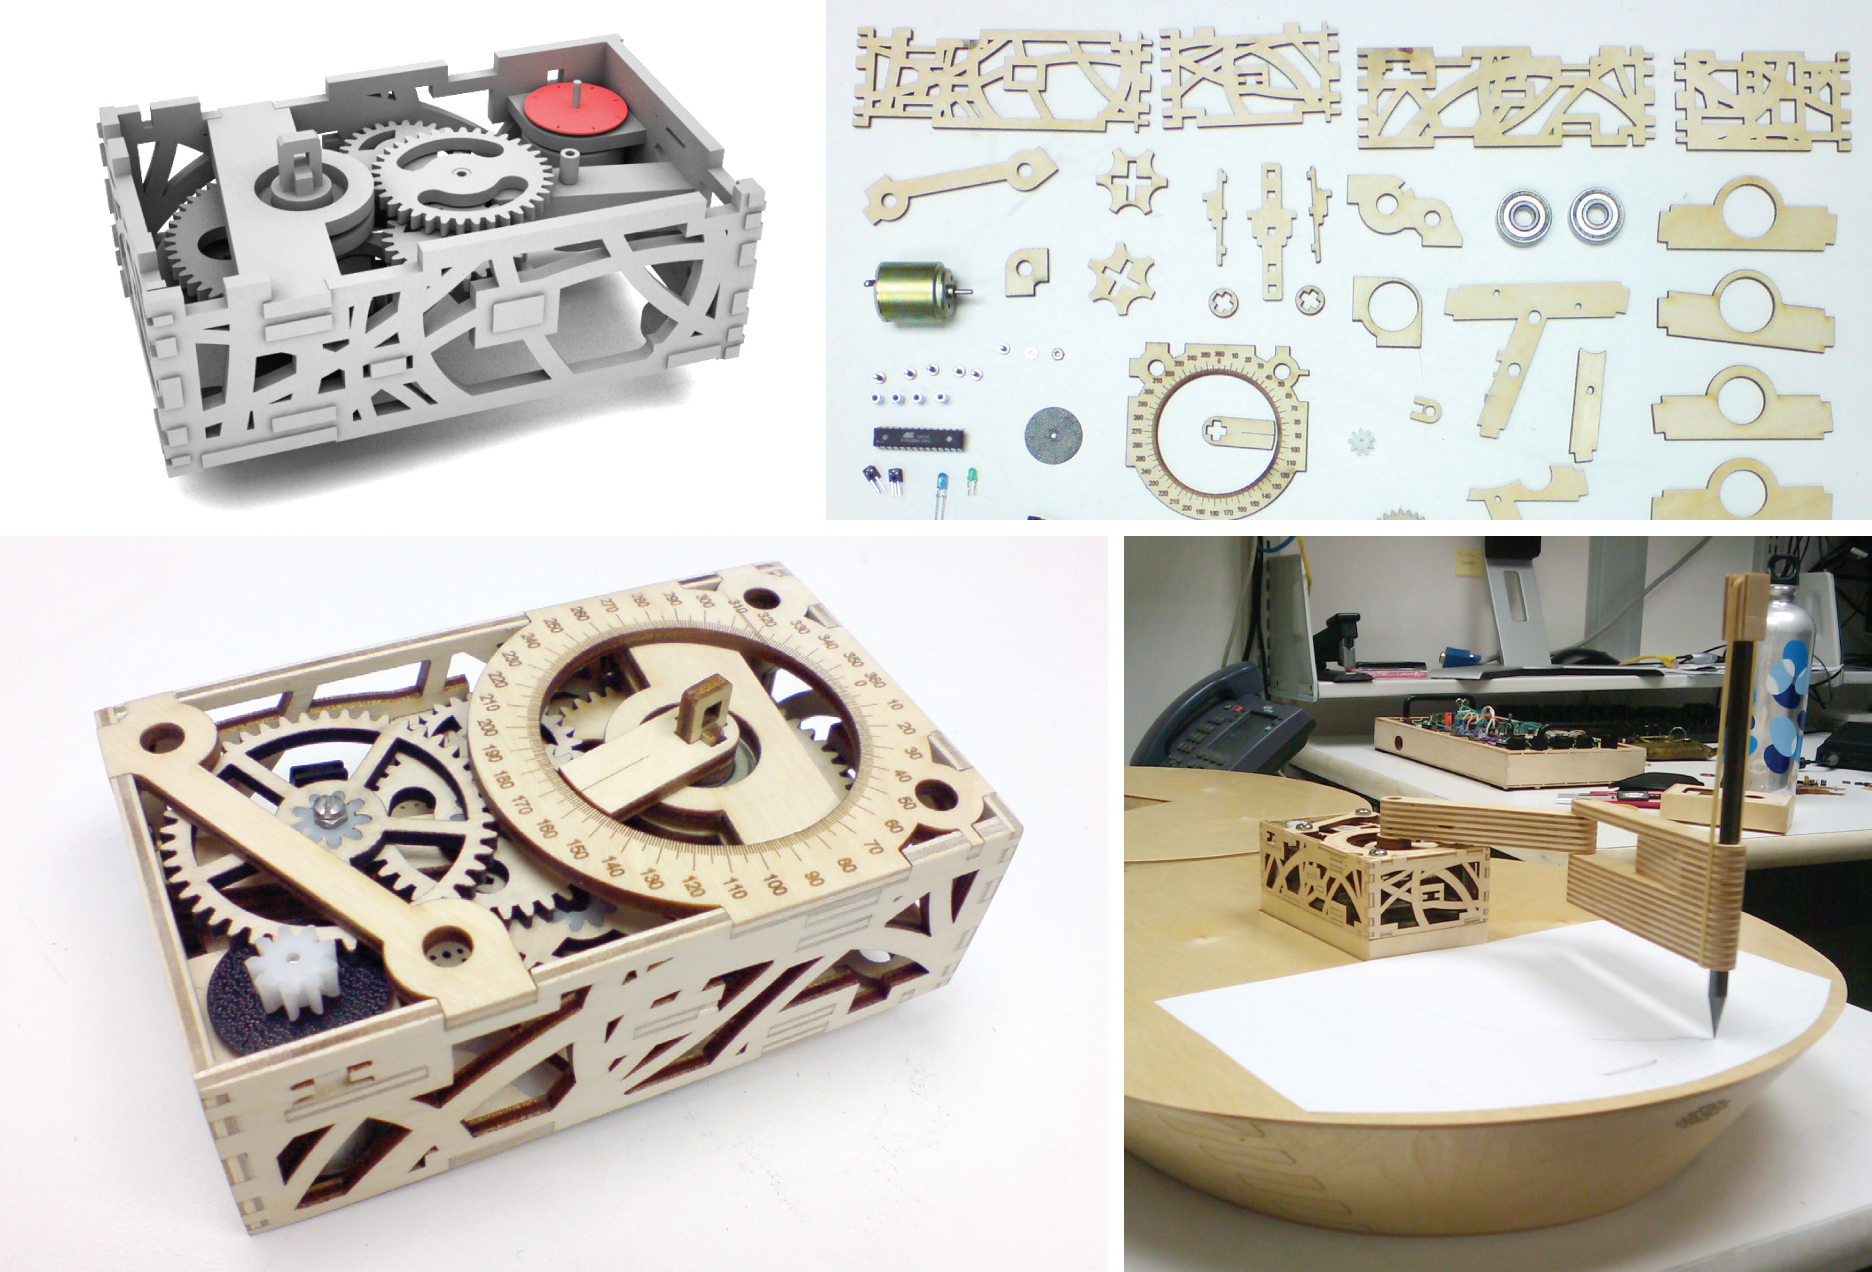
\includegraphics[width=\columnwidth]{images/plywood_servo.jpg}
\caption{Plywood Servo by Peter Schmitt (2011). (Clockwise from upper-left: 3d CAD model of partially constructed servo, laser cut plywood parts and electronic components, Audiograph, completed servo.)}
\label{fig:plywood_servo}
\end{figure}
\end{center}

\subsection{Computational Design and Craft}
Similar to artifacts developed through digital fabrication and craft, the combination of computational design and craft also offers the opportunity to produce pieces that are connected to a distinct space, time and process, and shaped by material properties, while incorporating patterns and forms made possible through computational processes. The Random Number Multiple series was a project that produced screen prints from the work of computational designers and artists. Figure \ref{fig:thorpe_screenprint} shows a screen print translation of the computational artist Jer Thorpe's RGB- NYT word frequency piece. The original piece was a digital image, which was generated from data on the usage of the words �red', �green', �blue' in the New York Times between 1981 and 2011. In translating the digital piece to physical form the result is distinct physical object, transformed by the material properties of screen printing. The artist describes the process on his website:

\begin{quotation}\textit{``This print turned out even better than I could have expected. The fine detail is amazing, the colours are rich and vivid, and the half-toning on the individual bars creates a jewel-like halo in the center that is fascinating to look at up close..This print was made with a semi-reflective ink, so it has a unique shimmer to it when viewed in the light."}
\end{quotation}

The rich material qualities Thorpe describes would be difficult to achieve by relying solely on a digital medium. In addition Thorpe describes pleasure he experienced in working with the tactile process of screen printing, and how the experience provided important creative feedback for his computational work \cite{thorpe_website}. 

\begin{center}
\begin{figure}[h!]
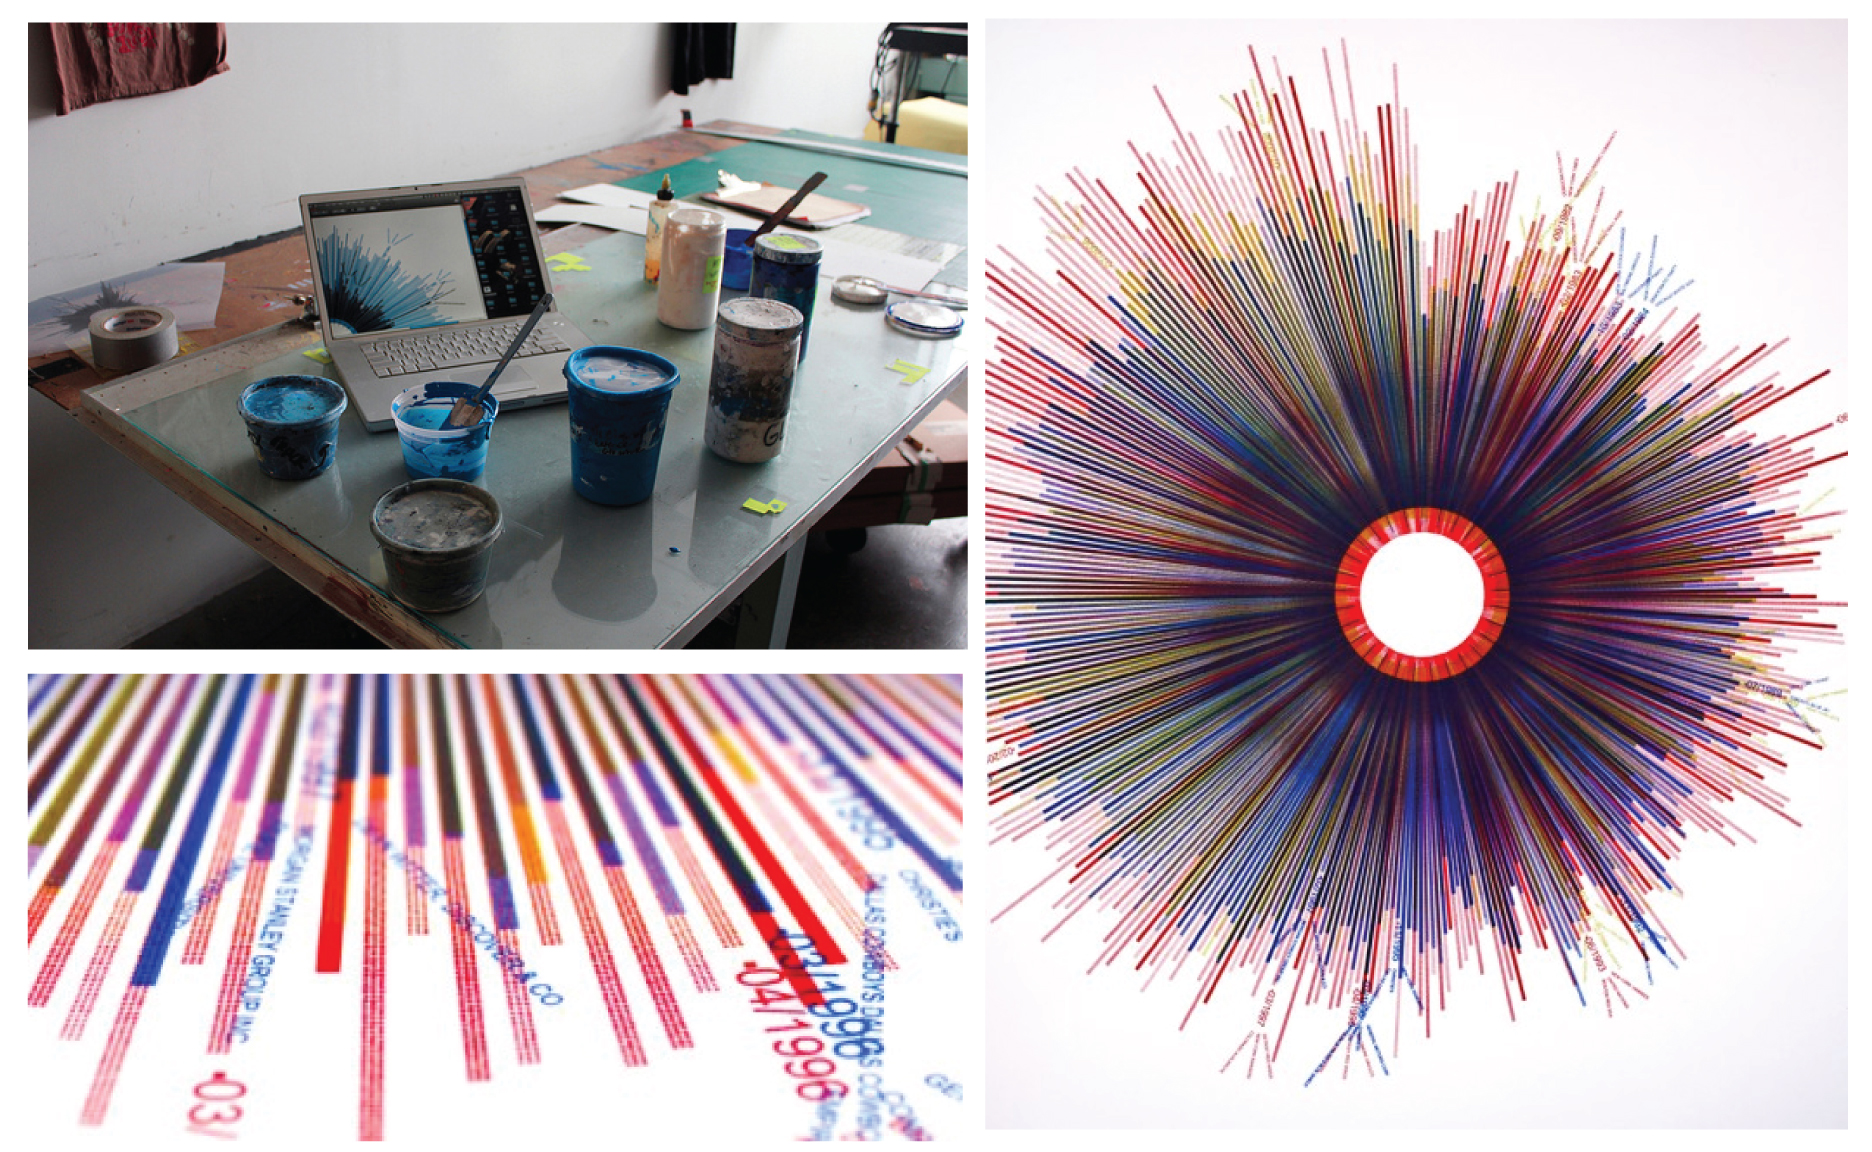
\includegraphics[width=\columnwidth]{images/thorpe_screenprint.jpg}
\caption{RGB � NYT Word Frequency by Jer Thorpe (2011). Part of the Random Number Multiples Series. Screen Print. (Counter-clockwise from upper-left: matching paint color to the digital image, close up of print, complete print.)}
\label{fig:thorpe_screenprint}
\end{figure}
\end{center}
\vspace{-20pt}

Combining computational design and craft also offers the opportunity to engage craftspeople in the use of computational tools. The Processing quilt (figure \ref{fig:processing_quilt}, was the result of a collaboration between Libs Elliott, a seamstress and quilt-maker, and Joshua Davis, a computational designer. Elliott created the quilt based on a processing program created by Davis which generated random triangle compositions. Elliott selected one specific composition and manually translated it to a grid and cut out the necessary pieces, and crafted a completed quilt (figure: \ref{fig:processing_quilt})\cite{elliott_website1}. 

\begin{center}
\begin{figure}[h!]
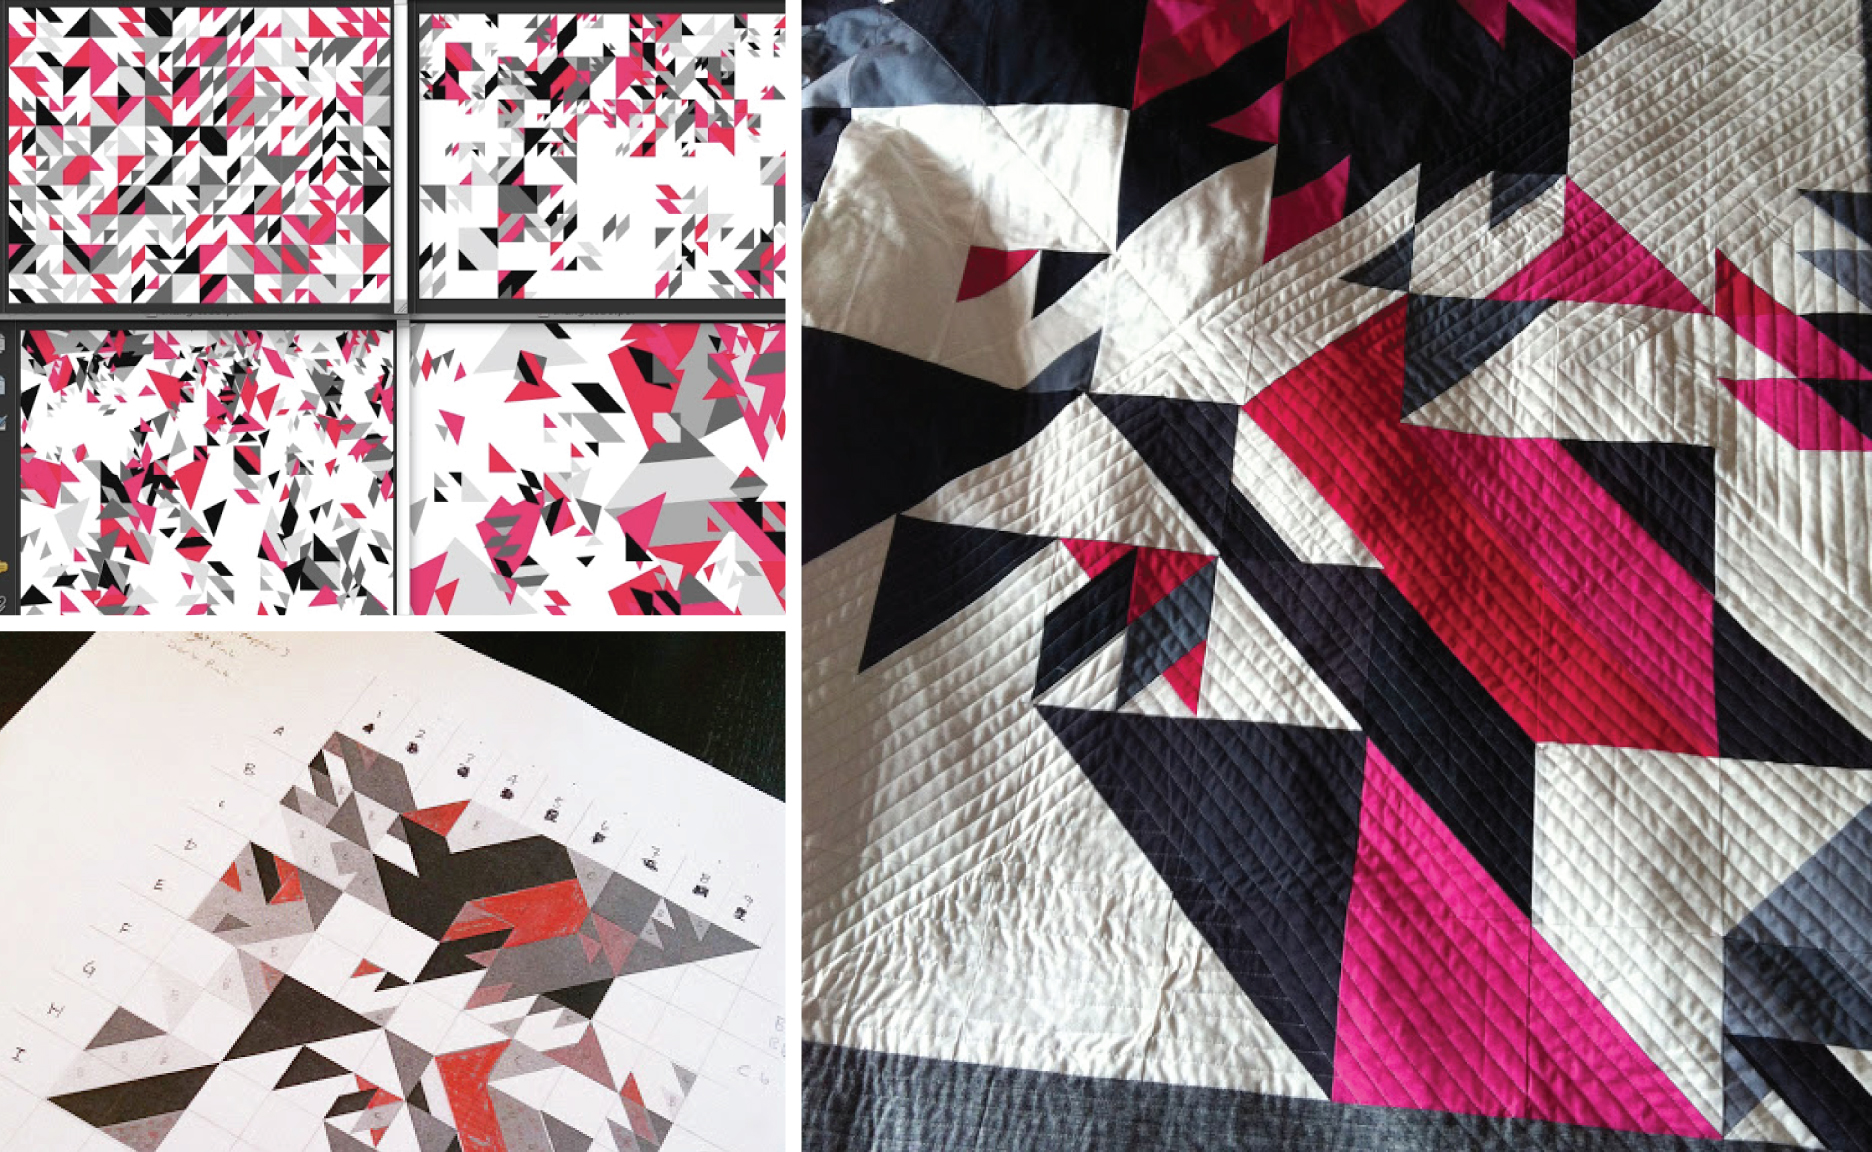
\includegraphics[width=\columnwidth]{images/processing_quilt.jpg}
\caption{Processing Quilt by Libs Elliott and Joshua Davis (2013). (Counter-clockwise from upper-left: auto-generated triangle compositions in Processing, hand-made quilt grid, Finished quilt.)}
\label{fig:processing_quilt}
\end{figure}
\end{center}

The resulting artifact is synthesis between computational aesthetics of the triangle composition, and the texture created by the quilted pattern. The piece exhibits the skills of Elliott and the computational expertise and style of Davis. The transition between computational forms and craft processes can be a source of frustration however. On her website, Elliot remarked about the contrast between working with a computational tool and producing something by hand:

\begin{quotation}\textit{``I'm not going to lie- quilting is a slow process and there's a certain level of frustration I have when I'm doing it. It's difficult to take something that works so quickly, like the Processing tool, to generate a hundred random compositions within an afternoon then force yourself to pick one image and slow it all down to an entirely manual process that takes days to produce \cite{elliott_website2}.}
\end{quotation}

The contrast in execution time between computational design and hand craft can be addressed by the introduction of digital fabrication. By combing all three of computational design, craft and digital fabrication into a single creative process, practitioners can more easily translate the qualities of of computational forms (including complexity, generativitiy, and precision) to physical form in a variety of materials. These physical forms in turn can be shaped through craft processes, and imbue computational designs with individuality, and utility. Several forms of digital fabrication machines are capable of producing forms that are suitable for both expert and novice levels of handcraft. Because subtractive fabrication technologies work with materials like wood, paper and fabric, they support the creation of objects that are readily shaped by the human hand. Laser cut parts can be sanded, polished, painted, sewn or folded after they emerge from the machine. Vinyl cutters can also be used on cloth and paper. They can also produce patterns in adhesive vinyl that can be applied to screens for for screen printing. Laser cutters and vinyl cutters also fabricate at a much faster rate than 3d printers or milling machines, and therefore results in a higher tolerance for error during the craft process; it is feasible to quickly re-cut damaged parts. 


\section{Challenges in broad participation in computational design and digital fabrication}
Through its association with hobbyist culture, many people consider certain forms craft to be accessible, and open to amateurs. Conversely, the combined use of computational design and digital fabrication is largely limited to experts and professionals. There are many practical barriers to novice participation in this domain. Most prominently, many of the programing languages used for computational design are difficult for novices to learn. In addition, a complex and convoluted process is required to translate a code-based design to a format that is compatible with fabrication machines \cite{gershenfeld}. Furthermore, the engineering challenges involved in designing complex objects from multiple digitally fabricated parts are extremely difficult to tackle for amateurs who are unfamiliar with CAD software. Although novice oriented CAD software exists, most of this software does not support computational design. Similarly, most novice oriented programing environments cannot produce designs that are suitable for fabrication on their own. 

There are also significant perceptual barriers to participation. There persists among the general public a limited perception of the applications of programing. Many people consider programing to be irrelevant to their interests, and therefore lack motivation to pursue what they perceive to be a highly specialized and difficult undertaking \cite{resnick1}. There are also perceptions of digital fabrication which may hinder creative and open use of these tools. Personal fabrication technology is often portrayed as a precursor to the production of replicator-like technology which can instantiate literally anything by building it directly from atoms \cite{gershenfeld}. This view can also act as a barrier to widespread engagement with existing forms of digital fabrication, by setting up unreal expectations for this technology,or by portraying it as a variation on traditional forms of consumerism. The idea of fabrication as a perfect replication system also eliminates the need or desire for human engagement in the fabrication process, eliminating the entry points for craft. Daniella Rosner describes this view in her research:

\begin{quotation}
 \textit{A central element of these and other visions of the future is that craft is done for us: Kitchens tell us what and how to cook, eliminating the creativity and pleasure of cooking from scratch with what's on hand; object printers create flawless prototypes, eliminating messily glued-together chipboard and toothpicks. In this new 
world, craft becomes fetish�the proudly displayed collection of vinyl records shelved alongside an iPod and digital files \cite{rosner_craft_vs_design}.}
\end{quotation}

Algorithmic fabrication is an exceptional form of creation. Through the unification of computational design, digital fabrication and hand production, one can create functional, beautiful and unique objects. If we are to extend practice of algorithmic craft beyond people with formal training in computer science and CAD, however, it is necessary to create accessible and open tools for programing and digital fabrication. These tools must be supported with practices that foster an understanding of the principles of computation, craft and digital fabrication and how they can be applied towards personal creative pursuits. 


